\documentclass[12pt,oneside]{report}

% \AddToHook{cmd/section/before}{\clearpage}

\usepackage[T1]{fontenc}

\usepackage{aas_macros}
\usepackage[letterpaper, top=1in]{geometry}
\usepackage{titlesec}

\titleformat{\chapter}{\normalfont\normalsize\centering}{Chapter \thechapter:}{1em}{}
\titleformat{\section}{\normalfont\normalsize\centering}{\thesection}{1em}{}
\titleformat{\subsection}{\normalfont\normalsize\centering}{\thesubsection}{1em}{}
\titlespacing*{\chapter}{0pt}{0pt}{40pt} \titlespacing*{\section}{0pt}{0pt}{20pt}
\renewcommand{\contentsname}{Table of Contents}
\AtBeginDocument{
      \renewcommand{\bibsection}{\chapter*{\bibname}}
  }

\usepackage{setspace}

\usepackage{etoolbox}% http://ctan.org/pkg/etoolbox
\makeatletter
% \patchcmd{<cmd>}{<search>}{<replace>}{<succes>}{<failure>}
\patchcmd{\@chapter}{\addtocontents{lof}{\protect\addvspace{10\p@}}}{}{}{}% LoF
\patchcmd{\@chapter}{\addtocontents{lot}{\protect\addvspace{10\p@}}}{}{}{}% LoT
\makeatother

\usepackage{amsmath}	% Advanced maths commands
\usepackage{txfonts}
\usepackage{hyperref}
\hypersetup{
    colorlinks=true,
    linkcolor=black,
    filecolor=black,
    urlcolor=black,
    citecolor=black,
    pdftitle={Thesis},
    pdfpagemode=FullScreen,
}
\urlstyle{same}
% \usepackage{amssymb}	% Extra maths symbols

\usepackage{graphicx}	% Including figure files
\graphicspath{{../figures/}}

\usepackage{natbib}
\usepackage[nottoc,numbib]{tocbibind}
% \usepackage[titles]{tocloft} % fig titles
% \renewcommand{\cftfigpresnum}{\figurename\enspace}
% \setlength{\cftfignumwidth}{5em}
% \renewcommand{\cfttabpresnum}{\tablename\enspace}
% \setlength{\cfttabnumwidth}{5em}



% \usepackage{fancyhdr}
% \pagestyle{fancy}
% \fancyhead{}
% \fancyhead[RO,RE]{Carbon Galactic Nucleosynthesis}
\pagestyle{plain}
\counterwithout{figure}{chapter}
\counterwithout{table}{chapter}




\defcitealias{cristallo+11}{C11}
\defcitealias{cristallo+15}{C15}
\defcitealias{ventura+13}{V13}
\defcitealias{karakas10}{K10}
\defcitealias{KL16}{KL16}
\defcitealias{karakas+18}{K18}



\newcommand{\cristallo}{\citetalias{cristallo+11}+\citetalias{cristallo+15}}
\newcommand{\karakas}{\citetalias{karakas10}}
\newcommand{\kl}{\citetalias{KL16}+\citetalias{karakas+18}}
\newcommand{\ventura}{\citetalias{ventura+13}}

\newcommand{\VICE}{\texttt{VICE}}
\newcommand{\caah}{[C/Mg]-[Mg/H]}
\newcommand{\caafe}{[C/Mg]-[Mg/Fe]}

\newcommand{\zoo}{\ensuremath{Z/Z_{\sun }}}
\newcommand{\Ycc}{\ensuremath{y_{\rm C}^{\rm cc}}}
\newcommand{\Yct}{\ensuremath{y_{\rm C, 0}^{\rm tot}}}
\newcommand{\Yoc}{\ensuremath{y_{\rm O}^{\rm cc}}}
\newcommand{\Ycagb}{\ensuremath{y_{\rm C}^{\rm agb}}}
\newcommand{\sun}{\ensuremath{\odot}}



\title{Carbon Nucleosynthesis}
% The list of authors, and the short list which is used in the headers.
% If you need two or more lines of authors, add an extra line using \newauthor
\author{Daniel A. Boyea}

% These dates will be filled out by the publisher
\date{\today}

\pagenumbering{roman}

\begin{document}

%\doublespacing


\begin{titlepage}
   \begin{center}
       \vfill
       \textbf{The Galactic Chemical Evolution of Carbon} \\
        Implications for nucleosynthesis
        \vfill
        Research Thesis
        \vfill
        Presented in partial fulfillment of the requirements for graduation \textit{with research distinction} in Astronomy and Astrophysics in the College of Arts and Sciences of The Ohio State University.
        \vfill
        by 
        \vfill
       {Daniel Alexandra Boyea}\\
       \vfill
       Department of Astronomy\\
       The Ohio State University\\
       \vfill
       April 2023
       \vfill
       Thesis Committee:\\
       David Weinberg, Advisor \\
       Jennifer Johnson \\
       Rolando Vald\'es Aguilar\\
       \vfill
            
   \end{center}
\end{titlepage}



% Abstract of the paper
\chapter*{Abstract}
\addcontentsline{toc}{chapter}{Abstract}
Stellar evolution models provide highly uncertain predictions for elemental yields due to our limited understanding of stellar physics. In this paper, we aim to estimate the nucleosynthetic yields of carbon using galactic chemical evolution models. 

We find that the AGB stars make up a fraction $0.20_{-20}^{+80}$ of total carbon production at late times. 

\chapter*{Acknowledgements}
\addcontentsline{toc}{chapter}{Acknowledgements}

James Johnson, for guiding me through this project and through my last year of undergraduate.
Wayne Schlingman, for everything you do for everyone. You are the glue holding together our department.
David Weinberg and Jennifer Johnson, for listening to my earlier drafts of this work and providing excellent suggestions.

I also would not have made it here without all the additional support from my friends and family. Eric, even across the country, you have always been a point of support and stability, and I am always happy to be around you. Anya, you are a wonderful friend and I cannot thank you enough for your support this year. 
I love so many people in our department who have just been friends and positive support: Kaia, Maria, Autumn, Simon, Mary, Aaliyah, Sanskruti, Alyssa, Harrison, Denis, and so many others. 
My Family (and Arya, our lovely doodle).


%% Lists

\tableofcontents
\listoffigures
\listoftables
\newpage
\pagenumbering{arabic}

%%%%%%%%%%%%%%%%%%%%%%%%%%%%%%%%%%%%%%%%%%%%%%%%%%

%%%%%%%%%%%%%%%%% BODY OF PAPER %%%%%%%%%%%%%%%%%%

\chapter{Introduction}


Astronomy is unique among sciences in that we can determine the history of chemical elements. While stable on earth, the churning gasses and firery stars can dramatically transform elements into new materials. However, we still have much to learn about how each chemical element is made. In this work, we will hope to clarify how the chemical element carbon, the basis of life, is made in the universe.

As the universe just began to cool following the big bang, the only elements around were hydrogen, helium, and trace amounts of lithium and berylium. All other elements were formed afterwords with the help of stars. Stars of different masses, ages, and metalicities have substantially different interior stuctures. Different stars produce vastly different amounts of different chemical elements depending on their properties. 

Stellar evolution, at the basis of galactical chemical evolution, predict the elemental production of different stellar processes. 
However, these models are rife with uncertainties, limited by our understanding of critical physical processes such as nuclear reaction rates, convection, opacity, and mass loss (CITE, e.g. stellar physics reviews). 

Carbon and nitrogen are well studied elements as they are easy to observe (Citations...). Additionally, carbon and nitrogen are used as age indicators for giant branch stars (citations, e.g. \cite{fiorenzo+21}), and are the only light elements known to be produced significantly in Asymptotic Giant Branch Stars (AGB) (cite).

However, our theoretical understanding of the producion sources of carbon are still uncertain.

While easily visible in many stars, determining birth abundances of carbon and nitrogen are 

One challenge of measuring abundances of carbon in star is that when a star becomes a RGB star, material from the CNO-processed core. Since this core-processed material is now carbon depleted and nitrogen enhanced, measurments of this star's atmosphere will no longer reflect the birth abundances of the star.
Additionaly, carbon is extremelt challenging to measure gas-phase abundances for because the strongest visible line is ...., e.g. carbon unreliable in GALAH, low detections.

AGB stars are known to be importaint (cite) from stellar model predictions, previous GCE, and evidence from abundance patterns. (are there detections in PN?)

CCSne are also important (.... SN reminant measurments)

We also know that there is evidence for non-monatonic carbon yield patterns. 
pattern where carbon is more readily produced by both high metallicity and very low metallicity stars (CEMPS, early GCE results), but our picture.

Additionally, stellar models are computationally expensive, even in one dimension, so while there are grids of predictions, these are not always fine enough to make accurate chemical evolution models. 


In Fig. \ref{fig:subgiants} we present a sample of APOGEE subgiants. These subgiants were chosen based on their location in the HR diagram based on criteria in \citet{jack_subgiant} replicated in Appendix \ref{sec:jack}. Because subgiants have not undergone FDU, their surface abundances are an accurate reflection of the birth abundances (CITATION).  




\begin{figure}[htp]
    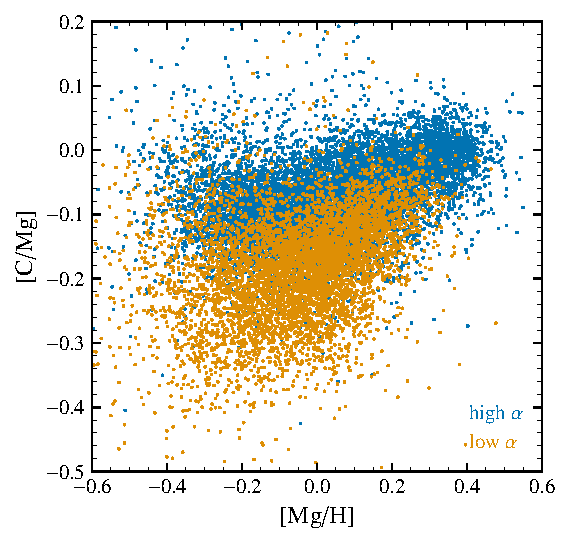
\includegraphics{subgiants_mgh.pdf}
    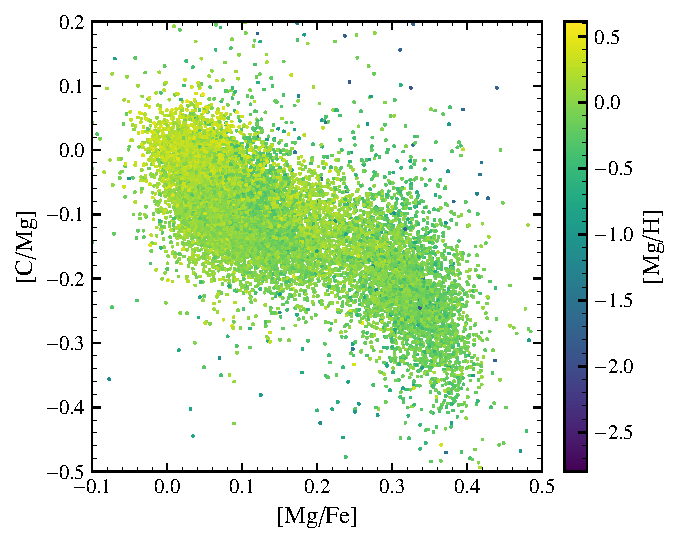
\includegraphics{subgiants_mgfe.pdf}
    \caption[APOGEE Subgiants]{The [C/Mg] ratio against [Mg/H] (left) and [Mg/Fe] (right) for the sample of subgiants as in \cite{jack_subgiant}. The left panel uses blue and orange to represent high and low $\alpha$ sequences respectively. On the right, we plot more metal rich ([Mh/H]) stars with darker colors.}
    \label{fig:subgiants}
\end{figure}
\chapter{Nucleosynthesis}

Nucleosynthetic predictions 
Modern theoretical nucleosynthesis provides our starting point for our models.  We focus on three primary nucleosynthetic pathways: AGB stars, CCSne, and SNeIa. Each process has unique timescales and element production which we can trace through the tools of GCE. While carbon is only known to be produced in AGB stars and CCSNe, comparing carbon to iron production (from SNeIa) adds a valuable constraint to our models and insight into the delay-time production of carbon.

After a group of stars are formed, CCSNe from massive stars are the first enrichment, providing light elements such as C, O, and Mg and heavier elements such as Fe and beyond. Importaintly, $\alpha$ elements like O and Mg are only formed in CCSNe (in significant quantities). Next, low mass stars begin to reach the end of their lives. The dying breaths of AGB stars are known to be importaint sources of C, N, and a smattering of heavier elements.  Finally, the white dwarfs, including formation and time to collide/over-eat, explode, releasing much of Fe and nearby elements. 

We focus on O and Mg as $\alpha$ elements only formed in CCSNe, and use Fe to
trace delayed enrichment from SNeIa. C and N are both formed in AGB and CCSNe.

There are two $\alpha$-elements we care about: Mg and O. Stellar observations
of magnesium are more reliable but oxygen abundances are easier to measure in
HII regions. We assume that both Mg and O are produced entirely in CCSNe with
constant, metallicity-independent yields. Thus $\text{[Mg/H]} = \text{[O/H]} =
[\alpha/\text{H}]$ in our models. (Observational validation?)

For carbon, the dominant producer is from massive stars which eject carbon fused in their cores during CCSNe. 

As we focus on the yields of carbon, we keep yields for other elements fixed in
most models. Taken from \citet{james+21, james+22}, we let
\begin{itemize}
    \item $Y_\text{O}^\text{CC} = 0.015$
    \item $Y_\text{O}^\text{Ia} = 0$
    \item $Y_\text{Fe}^\text{Ia} = 0.00214?$
    \item $Y_\text{Fe}^\text{CC} = 0.0012$
    \item $Y_\text{N}^\text{CC} = 0.00036$
    \item $y_\text{N}^\text{AGB}(M, Z) = 9\times 10^{-4} M \left(\frac{Z}{Z_\odot}\right)$
\end{itemize}
Also following \citet{james+21, james+22}, we take the SNeIa Delay Time distribution to be a
$t^{-1.1}$ law suggested by the observations of \citet{maoz+12}.


\section{Asymptotic giant branch carbon}

\begin{figure*}
    \centering
 	    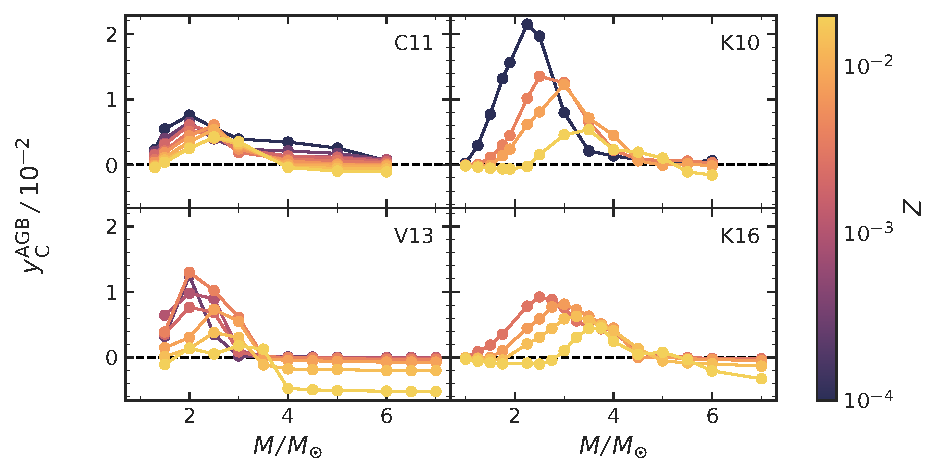
\includegraphics[scale=1]{agb_yields.pdf}\\

        \caption[AGB carbon yields]{The net fraction carbon yield ($M_\text{C}$, the amount of carbon produced by the star divided by $M$) plotted as a function of mass, $M$. Lighter colors represent higher values of metalicity ([M/H]). Each panel represents a different AGB model. K10 reports stars at MoverH -3, -2, etc. I can reproduce C11 and K10 but not other V13 and KL16 :(((}

    \label{fig:y_agb}
\end{figure*}

\begin{figure}
    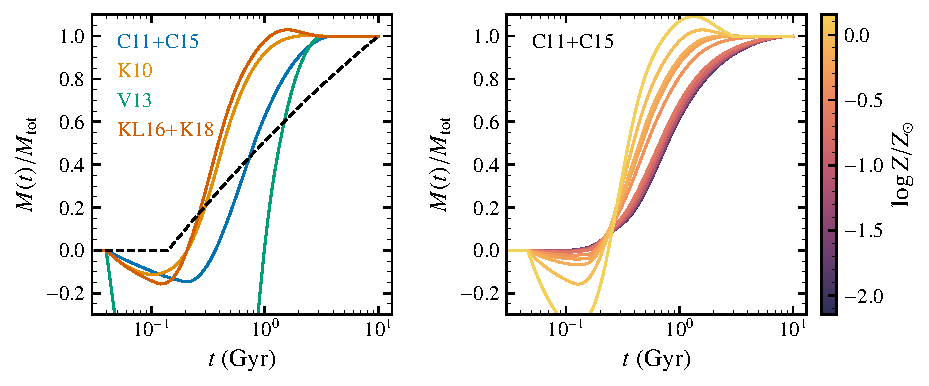
\includegraphics[scale=1]{y_agb_t2.pdf}

    \caption[AGB DTD]{
    The Delay Time Distribution for AGB STars}

\end{figure}

\begin{figure*}
    \centering
    
    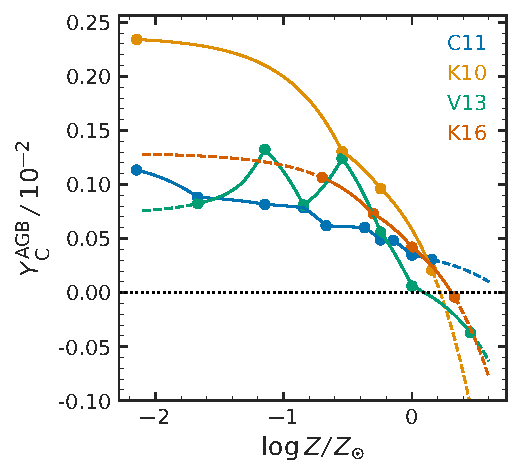
\includegraphics[scale=1]{y_agb_vs_z.pdf}

    \caption[SSP AGB carbon]{On the left, we plot the IMF weighted net fractional carbon yields of each AGB model as a function of metalicity.The right panel plots the normalized net carbon AGB yield as a function of time for a population of stars born at the same time at solar metallicity. We note that for the right panel, the minimum of the DTD for V13 is }

\end{figure*}

An AGB star is a low mass ($\lesssim 8 M_{\sun}$) star during the final phases of evolution.  In an AGB star, two competing processes determine the outcome of carbon production.
Third Dredge Up (TDU) is needed to eject carbon from the star, enriching the surface with helium-burning-processed material from the core. But Hot Bottom Burning (HBB) at the base of the convection layer changes carbon into nitrogen. 
TDU occurs during thermal pulsations, where the convective layer of the star passes into the inner layers with He-burning products which mixes in C and O into the envelope. In contrast, HBB may happen if the base of the convective envelope reaches about 50MK, initiating the CNO cycle, converting most C12 into N14. 

Carbon abundances are strongly affected by CNO cycle processing in stars. The CNO cycle is one of two series of nuclear reactions( $^{12}$C(p, $\gamma$)$^{13}$N($\beta^+ \nu_e$)$^{14}$N(p, $\gamma$)$^{15}$O($\beta^+\nu_e$)$^{15}$N(p,$\alpha$)$^{12}$C

Because the $^{14}$N(p, $\alpha$) proton capture is the slowest component of the CNO cycle ****, the CNO cycle, to first order, converts all $^{12}$C into $^{14}N$. 

The differences in yields between AGB models depend on the mass loss rate, treatment of convection, and nuclear reaction rates. 

In this work, we explore four different sets of AGB star yields representative of the variety of options which also provide reasonably well sampled grids in metallicity and mass necessary for chemical evolution studies.
\begin{itemize}
    \item \citet{cristallo+11} and \citet{cristallo+15} (\cristallo).
    \item \citet{karakas10} (\karakas)
    \item \citet{ventura+13} \ventura
    \item \citet{KL16} \citet{karakas+18} \kl
\end{itemize}
Unless otherwise noted, C11 is the model we choose as our fiducial AGB yield. 

We use IMF-Integrated yields calculated with \VICE~throughout this paper (see
section \ref{sec:vice}, \citet{james+21, james+22}). For an element X and star
with mass $M$, the stellar yield $y$ is defined as the net production of X relative 
to $M$, or
\begin{equation}
    y_{\rm X} = \frac{M_{\rm X,\ ejected} - Z_{0, X} M_{\rm ejected}}{M}   
\end{equation}
where we let $M_{\rm ejected}$ and $M_{\rm X, ejected}$ be the total ejected
stellar mass (through winds and supernovae ejecta) and the ejected mass of X,
and $Z_{0, X}$ was the birth mass fraction of element X.

More useful for GCE are Initial Mass Function (IMF) yields, where we sum up the
contributions of all stars which produce an element.
We define the IMF-integrated yield of X with: 
\begin{equation}
Y_{\rm X}^{\rm proc}(Z) = \int_{M_{\rm min}}^{M_{\rm max}} y_{\rm X}^{\rm proc}(M, Z)\ \Phi(M)  \ dM
\end{equation}
Where $\Phi(M) = \frac{dN}{dM}/ \int_{M_{\rm min}}^{M_{\rm max}} \frac{dN}{dM}\ dM$ is the normalized IMF, $M_{\rm min}$ and $M_{\rm max}$ are the minimum and maximum mass of stars, which we take to be $0.08 M_{\sun}$ and $100 M_{\sun}$ respectively; and $\frac{dN}{dM}$ is the initial mass function, the frequency of stars born between $M$ and $M+dM$.


Fig. \ref{fig:y_agb} compares the net fractional AGB carbon yield, $m_\text{C}^\text{AGB}(M, Z)$ for each AGB model we consider. Note that the yields may be negative when the birth abundance is higher than the carbon abundance of the material ejected back to the ISM. 

Most models agree on the qualitative shape of the net fractional AGB carbon yield. The stars with the highest fractional carbon yields are between 2 to 4 solar masses, depending on the metallicity and model. Both lower and higher mass stars produce less carbon, and high mass stars may even destroy carbon at high metallicity due to highly efficient HBB. And all models agree that the carbon yield generally decreases with metallicity. 


Metallicity dependence:
V13 is the only model that stands out, showing a non-monotonic metallicity dependence, however this effect is only for models with [M/H]$\leq -1$. Otherwise the major differences between the models are the precise amount of carbon and the slope of the metallicity dependence. For example, the three models C11, K10, and K16 predict $y_\text{C}^\text{AGB}$ to be between 0.006 and 0.008 at solar metallicity, but C11 has a much shallower metallicity dependence than the K10 and K16 models. And at solar, V13 predicts a value at around 0.004 so the models are all within about a factor of 2. 

Another difference is the speed at which equilibrium is reached. K10 and K16 weight carbon production more heavily towards massive stars resulting in a faster time to equilibrium, whereas the C11 and V13 models predict a slightly longer timescale with order 1Gyr, but little to no carbon is produced more than 2Gyr after a star formation event. This is in contrast to iron which is still produced by SNeIa up to 10Gyr after a star formation event. 


\section{CCSNe carbon}

\begin{figure}[htp]
    \centering
    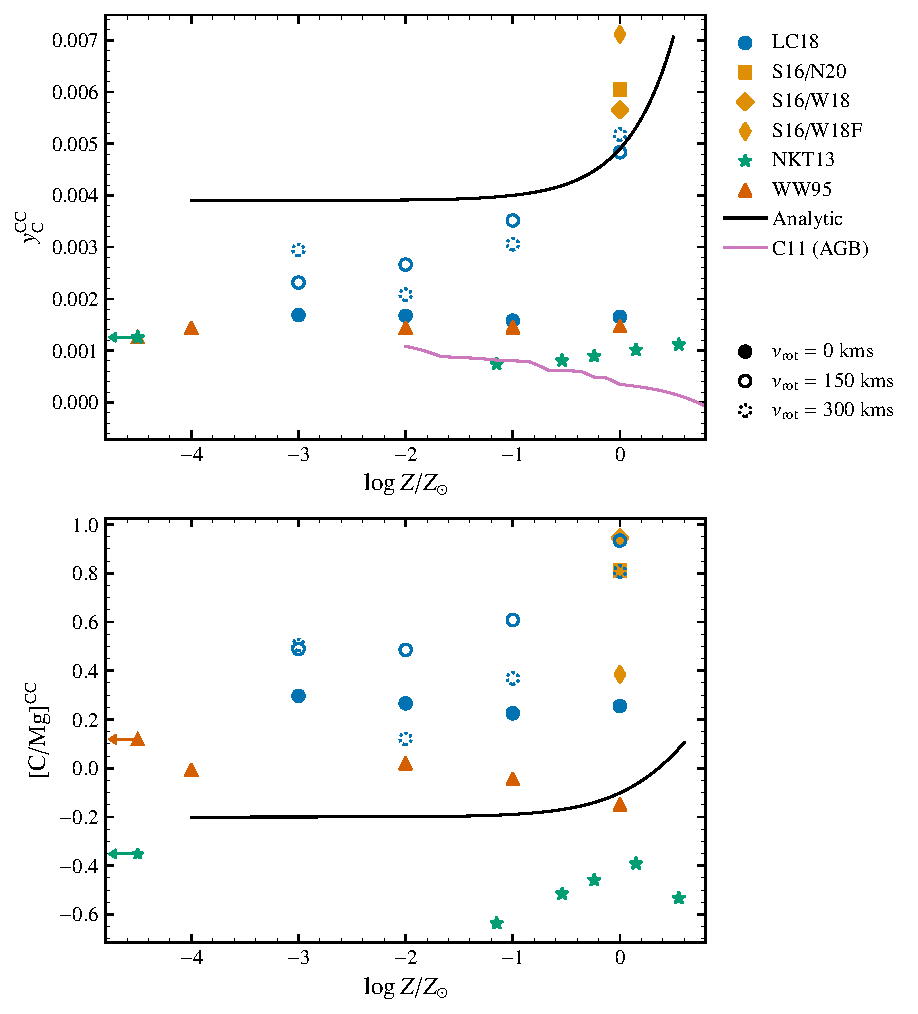
\includegraphics{y_c_cc.pdf}
    \caption[CCSNe carbon yields]{The fist plot shows IMF-weighted net fractional CCSNe yield of
        carbon, $y_C^{cc}$ against metalicity, [M/H], for different studies.
        The right plot instead shows [C/O]$^\text{CC}$, the logarithm of the
        abundance ratio of carbon to oxygen if CCSNe were the only carbon
        source, also as a function of metallicity for the same set of studies.
        The black line represents the carbon yield of the fiducial model,
        $y_C^{CC} = 0.004? (Z/Z_{\sun})^{0.3}$, and becomes dashed over regions
        where we have not tested our model.\citep{NKT13}, \citep{LC18},
        \citep{sukhbold+16}, \citep{WW95}
 }
    \label{fig:y_cc}
\end{figure}

Massive stars form $^{12}$C through the triple--$\alpha$ process. However, the carbon has to get out of the star to be useful. 
While there are many stellar models providing predictions of CCSNe yields, the results of these models are highly uncertain due to the many stellar modeling uncertainties. 

We summarise many of the predictions of stellar models in Fig. \ref{fig:y_cc}. 
\begin{equation}
    {\rm [C/O]^{CC}} = \log_{10}\left( \frac{y_{\rm C}^{\rm CC}}{y_{\rm O}^{\rm CC}}\right) - \log_{10} \left( \frac{Z_{C, \sun }}{Z_{O, \sun }} \right)
\end{equation}
Notice how even these ratios 



    \begin{itemize}
        \item Wide range in predictions, exacerbated to 1 dex range when including variance in oxygen predictions
        \item (explain) most models have a near-metallicity independent oxygen yield, so we choose the fiducial value of 0.015 despite varience in $y_O^{cc}$
        \item The fiducial value, where we choose the carbon yield from Sukhbold+16, may be above most predictions of carbon yields but is within the range of yield ratios
        \item the fiducial value would reach an equilibrium carbon yield of -0.1 without AGB stars
        \item Rotation in LC18 appears to increase metallicity dependence of carbon production (read this paper more carefully)
        \item NKT and LC agree in positive metallicity depenent yields
    \end{itemize}
    


\chapter{The Equilibrium Approximation}\label{sec:equilibrium}

Chemical abundances reach an equilibrium. New elements produced in stars balance the elements lost to galactic winds and inside stellar reminants. At the present day, our galaxy has evolved long enough to be well approximated by the chemical equilibriums. 

In equilibrium, if we know the yields, than the largest uncertainty is the rate of outflows. This determines the final abundances of evolutionary ... \cite{WAF17}. 

If we assume that the median track is an equilibrium phenomenon, we can calculate the total carbon to oxygen yield ratio. Additionally, assuming an AGB yield set enables us to predict the CCSNe carbon yield.  
We begin with the model, which underlies the multizone simulations, that the change in mass of an element is a sum of production, outflows, recycling, and mass left in reminants. We write this as
\begin{equation}
M_\text{C} = y_\text{C} \dot{M}_\star - (1 + \eta - r) Z_\text{C} \dot{M}_\star
\end{equation}

In the case that carbon
\begin{equation}
Z_c^{eq}(R) = \frac{y_c^{cc} + \langle y_c^{agb} \rangle }{1 + \eta(R) - r - \tau_\star / \tau_{sfh}}
\end{equation}Where
\begin{equation}
\langle y_c^{agb} \rangle = \frac{\int_0^T y_c^{agb}(M, Z) \dot{M}_\star(T - t) \frac{dN}{dM} \frac{dM}{dt} dt  }{ \dot{M}_\star \int_0^T \frac{dN}{dM} \frac{dM}{dt} dt}
\end{equation}

Likewise for oxygen:
\begin{equation}
Z_O^{eq}(R) = \frac{y_O^{cc}}{1 + \eta(R) - r - \tau_\star / \tau_{sfh}}
\end{equation}

However, for the yield ratio, the denominator cancles with that of oxygen, so the ratio is fixed.
\begin{equation}
\frac{Z_c^{eq}}{Z_o^{eq}} = \frac{y_c^{cc} + \langle y_c^{agb} \rangle }{y_o^{cc}}
\end{equation}

For this analysis, we let $y_c^{agb}$ represent the default AGB yields from a given yield set, but add a process factor $\alpha_{agb}$ which multaplicatively increases the AGB fraction. See Table \ref{tab:alpha_agb}.

\begin{equation}
    y_{\rm C}^{\rm CC} \rightarrow \alpha_{agb}  y_{\rm C}^{\rm CC}
\end{equation}

With these definitions, we can calculate the core collapse yields of carbon as a function of metallicity:
\begin{equation}
    y_\text{C}^\text{CC} =  y_\text{O}^\text{CC} \frac{Z_\text{C,eq}}{Z_\text{O,eq}} - \alpha_{agb} \langle y_c^{agb} \rangle
\end{equation}

Rewriting in terms of the observed abundance ratio and dividing by
$y_\text{O}^\text{CC}$. So, given the outflows or CCSNe oxygen yields, the
carbon AGB yield, and the \caah mean abundance track, we can estimate the CCSNe carbon yield. Written as a relative yield:
\begin{equation}
    \frac{y_\text{C}^\text{CC}}{y_\text{O}^\text{CC}} = \frac{Z_{C, \sun}}{Z_{O, \sun}} 10^{[C/O]} - \frac{\alpha_{agb} \langle y_c^{agb} \rangle}{ y_\text{O}^\text{CC}}
\end{equation}

This equation corroberates what we have explored earlier in the paper, and provides our analytic estimates of the CCSNe carbon yields. Since the AGB term is subtracted, a negative AGB Z-dependence will correspond to a positive CC Z-dependence. And as we reduce outflows, the AGB factor increases, steepening the required slope of the carbon yields. So, while the AGB yields may agree with eachother, the uncertainties in the oxygen CC yields and outflows leads to a substantial uncertainty in the AGB fraction.  

\begin{figure}
    \centering
    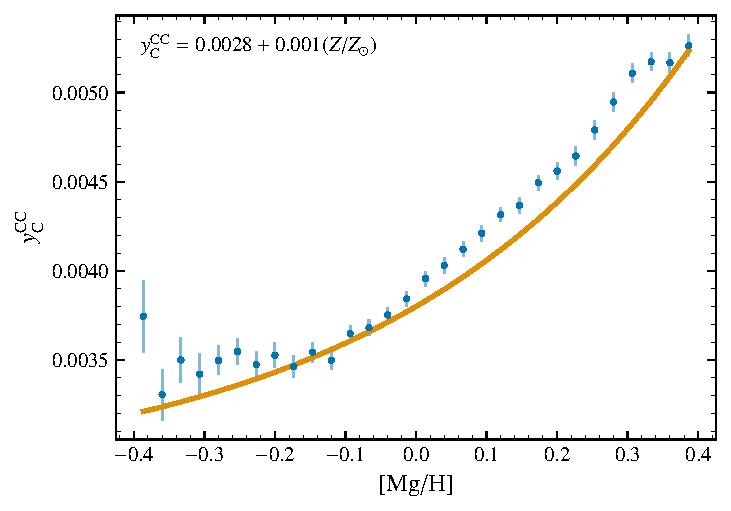
\includegraphics[]{analytic.pdf}
    \caption[Reverse fit yields]{Our reverse fitting method to determine total CCSNe contribution}
\end{figure}

% y_c^cc = (0.0148 +- 0.00016) Z^{0.154 +- 0.0053}
\begin{equation}
    y_C = (0.0029 \pm 0.0005) + (0.001 \pm 0.0004) \left(\frac{Z}{Z_\odot}\right)
\end{equation}

With uncertainties 

\section{Model Stellar Yields}
We define a parameterization of a CC~yield
  Because of the large uncertainties in CCSNe carbon yields, we choose to explore an analytic expression of the yield enabling us to easily explore how variations of CCSNe carbon yields affect abundance tracks. We find that a powerlaw yield with a metallicity-dependent constant minimum is able to match the observations well while remaining a simple parameterization (see below). Our expression is:
  \begin{equation}\label{eq:y_yields}
   Y_\text{C}^\text{CC}(Z) =  \alpha\ Z^\beta Y_\text{O}^\text{CC} + Y_\text{C, 0}^\text{CC}
    \end{equation}
   	Where we estimate $\alpha = 0.02$ and $\beta = 0.25$ (See Section \ref{sec:equilibrium} ). Our second model uses $\alpha = 0.44$ and $\beta = 0.63$ with K16 yields and reduced $\eta \rightarrow 1/2 \eta$ 
    
    As an overall scaling of yields does not significantly affect our models, we choose to fix the total equilibrium value of the total carbon yield at solar at $Y_{\text{C},\ \sun} = 0.005$, and then scale the yields relative to this value. 


\section{Uncertainties}

We only perform this analysis on the C11/15 yields because the range of metallicities of the data (about [M/H] = -0.4, 0.4) only represents about 2 AGB models, relying heavily on our choice of extrapolation. C11/C15 have a finer model grid, allowing us to have 5 theoretical predicted points within this metallicity range, allowing us to be more certain of our conclusion. 

We do note that this analysis fails to take into account selection effects and biases in APOGEE, and a more robust determination of the carbon yield. 


This formulation is degenerate in $\varpi$ until we estimate a better AGB fraction. As the seperation between the low and high alpha sequences can be used to estimate the delayed time contribution to carbon, using the model to estimate this value relies heavaly on the details of the SFH in addition to the 
We do give an estimate of the CCSNe yields, however this is dependent on our choice of $\eta$. Other choices of $\eta$ vary the value significantly in both magnitude and slope (as AGB contributions increase, we need less CCSNe carbon, however the CCSNe carbon must have a higher metallicity dependence to replicate the V21 data). 



\chapter{The Multizone Model}\label{sec:vice}

To simulate the chemical evolution of a Milky-Way-like galaxy, we use the Versitile Integrator for Chemical Evolution (\VICE\footnote{\VICE~is available at \url{https://github.com/giganano/VICE}}) published in \citet{james+21} and also briefly described in \citet{james+22}.  As a multi-zone model, the galaxy is divided into 200 rings of 0.1kpc, each with separate gas supplies with outflow and inflow rates. 


\VICE\ accounts for radial migration by using the results of the \texttt{h277} hydrodynamical simulation. Each VICE SSP is matched to a random nearby star particle \textit{analogue} in \texttt{H277}. VICE approximates the migration of this particle by using a $\sqrt{\text{time}}$-diffusion approximation where the change in galactic radius of a star, $\Delta R$, is $\Delta R \propto \sqrt{\text{t}}$. 
VICE does not account for radial gas flows. 

Other approaches have used dynamical arguments to implement their stellar mirgrations. We note that our approach does not introduce more free parameters which may bias conclusions. However, we only consider one dynamic history, and it is still unknown how variations in the dynamic history of a galaxy impact its chemical evolution.


We initially assume an "inside-out" SFH where the star formation rate peaks in the early evolution of the galaxy and is higher closer to the galactic center. The star formation rate, $\Sigma_\star$, for our fiducial model is parameterized by
\begin{equation}
    \dot{\Sigma}_\star \propto \left(1-e^{-t/\tau_{\rm rise}}\right) e^{-t/\tau_{\rm sfh}}
\end{equation}
where $\tau_\text{rise}=2$Gyr is the
and $\tau_{sfh}$ is the rate of decline of the star formation rate, which is based on *****.

We also explore a "lateburst" model which is parameterized with a normal distribution multiplying our fiducial "inside-out" SFH as
\begin{equation}\label{eq:lateburst}
    \dot{\Sigma}_{\rm lateburst} \propto \dot{\Sigma}_{\rm insideout} \left(1 + A e^{-(t-\tau_{\rm burst})^2/2\sigma^2_{\rm burst}} \right)
\end{equation}

$A=1.5$ represents the amplitude of the birth, $\tau_\text{burst}=10.8$Gyr is the time where the burst is strongest, and $\sigma_\text{burst}=1$Gyr is the width of the burst. We do explore the effects of variations of this parameterization in section ****.


VICE normalizes the total mass of star formation against observations from ******.
The gas inflow is calculated based on our star formation parameterization by using a schmit law 
\begin{equation}
    dM_g \propto \dot{\Sigma}^{1/n}
\end{equation}
where we take $n$ to be ****

Salpeter IMF.


\chapter{Multizone model results}
\section{Data Selection}

We use data from APOGEE DR17 \citep{apogee17} processed with APOSCAP. Since subgiant stars have yet to experience FDU, their atmospheric carbon and nitrogen abundances are still reflective of their birth abundances and do not need mixing corrections. 

To select for subgiants, we use the following cut in $\log g$ and $T_{\rm eff}$
which selects stars at the base of the red giant turnoff (FIGURE and
\cite{jack_subgiant}). We describe our selection criteria along with a 
comparison to \citet{fiorenzo+21} in Appendix \ref{sec:jack}. 

Because the star formation history is left in a simple inside-out form, this multizone model does not reproduce the high-$\alpha$ sequence, therefore we make the following cut to the V21 data to remove the high alpha sequence.

\begin{equation}
\begin{cases}
\text{[Mg/Fe]} >0.12-0.13\text{[Fe/H]}, & \text{[Fe/H]}<0\\
\text{[Mg/Fe]} >0.12, & \text{[Fe/H]}>0\\
\end{cases}
\end{equation}




\section{The Evolution of carbon across the galaxy and through time}

\begin{figure*}
\label{fig:c_evo}
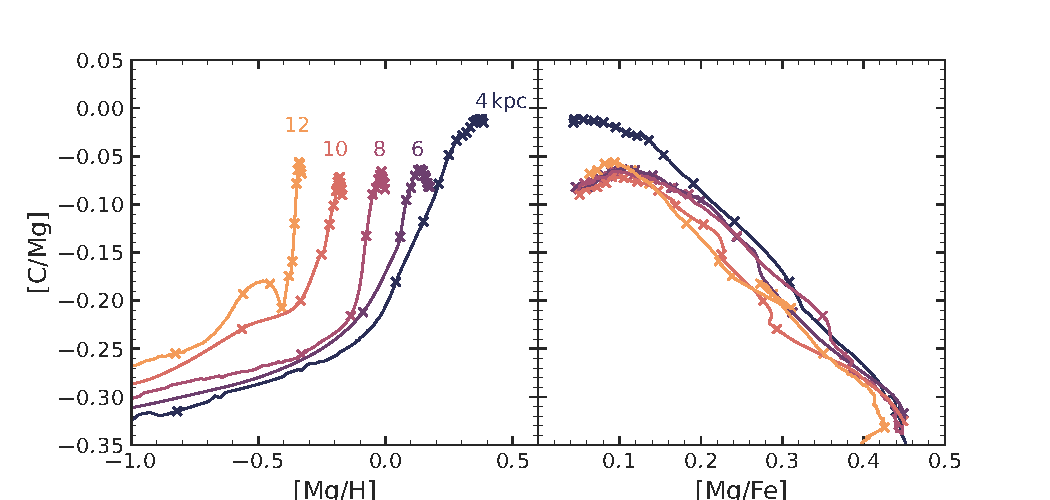
\includegraphics{evo_tracks.pdf}
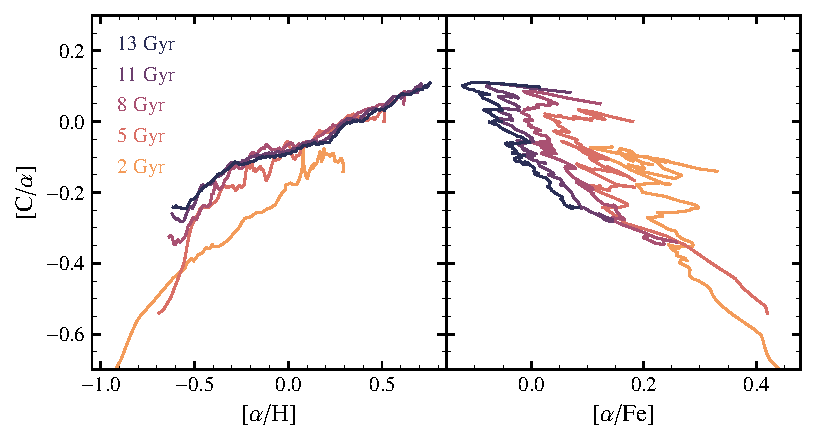
\includegraphics{evo_slices.pdf}
\caption[Carbon chemical evolution tracks]{The top set of panes show the time evolution of the gas phase of our
    fiducial model, plotted as tracks through \caah and \caafe where each colored line corresponds to the evolution at that galactic radius. 
The bottom set instead shows the galaxies gas-phase \caah and \caafe trend at 5 different time slices. 
}
\end{figure*}

Here, we present our fiducial model which we will later show aggrees well with APOGEE. We will later investigate the effects of alterations to this model. 

In this model, we use the following yields:

The GCE of carbon is complicated by metallicity dependencies and delayed contributions. 

We note the following features of our model:

\begin{enumerate}
    \item Carbon comes predominantly ($\sim80\%$) from CCSNe but the rest is from AGB stars
    \item The CCSNe carbon production is more efficient at higher metallicities
    \item AGB stars produce less carbon at higher metallicities.
\end{enumerate}


The combination of these features leads to an evolution that proceeds as follows
\begin{enumerate}
    \item Initially, CCSNe dominate production before AGB stars can contribute their enrichment, but because CCSNe is highly metalliticy dependent, the C/$\alpha$ ratio increases with time.
    \item AGB stars begin contributing their carbon, increasing the $C/\alpha$ ratio more steeply as the gas begins to reach its equilibrium metallicity
    \item When $Z$ reaches equilibrium, the $C/\alpha$ ratio stops increasing or may even decline, as AGB stars formed at higher metallicities reduce the net carbon yields.
\end{enumerate}

We plot time evolution tracks in Fig. \ref{fig:c_evo} for \caah and \caafe for our fiducial model. Comparing [C/$\alpha$] against [Fe/H] enables us to see late time evolution of carbon more clearly. Because [Fe/H] takes longer to reach equilibrium as half of iron production comes from type-Ia supernovae, the late time evolution is not clustered as tightly horizontally as for [$\alpha$/H].
This is even more evident in the lower part of Fig. \ref{fig:c_evo}. While the \caah trend reaches almost equilibrium at 5Gyr, the \caafe trend continues to evolve even until the present day, exposing the effect of the delayed contribution from AGB stars on the evolutionary history.

\begin{itemize}
    \item Describe definition of $f$ /etc.
    \item How we match the figures, DTD vs $\zeta$

\end{itemize}


\begin{figure}
\centering
\includegraphics{oob_agb.pdf}

\caption[AGB GCE Models]{Left: the \caah~ \textbf{median} present-day stellar tracks for four different
AGB models (\cristallo, \karakas, \kl, and \ventura ). The median bin [C/Mg] values from \citet{jack_subgiant} are
plotted as black points with 1-std errors marked by horizontal grey dashes.
Right: same as left but for \caafe. While each AGB yield model may
differ in detail, there is minimal effect on the overall [C/Mg] trends.

While we show the entire dataset in Fig. \ref{fig:subgiants}, we chose to compare the
binned data to our models as black points with dashes representing the 1-sigma
spread, as in e.g. Fig. \ref{fig:agb_sims}. \label{fig:agb_sims}
}
\end{figure}

\section{Alternate Models}

What happens as we change our choice of AGB stellar yields? We consider four models
using the published yields in \cristallo, \karakas, \kl, and \ventura~in Fig.
\ref{fig:agb_sims}. 

As we chose to leave $Y_{\rm C}^{\rm CC}$ in a functional form, we chose to
leave the total IMF-averaged carbon yield to be constant. The magnitude of
$Y_{\rm C}^{\rm CC}$
\begin{equation}
    Y_{\rm C}^{0}  = 0.005  =  Y_{\rm C}^{\rm cc} + Y_{\rm C}^{\rm agb}
\Big \rvert_{Z=Z_\odot}
\end{equation}
where we are choosing to evaluate the total IMF CC and AGB yields at solar
metallicity. We show our calculations of $Y_{\rm C}^{\rm agb}(Z=Z_{\sun })$  in
Table \ref{tab:alpha_agb}. 

This choice of total carbon yield with our fixed choice of oxygen gives an
equilibrium value of $Z_{\rm C}/Z_{\rm O} = Y_{\rm C}/Y_{\rm O} = 0.333$ which
is reasonably consistant with the value in \citet{asplund+09} of $Z_{\rm
C}/Z_{\rm O}=0.413$ and was chosen as to match the median value of our sample
at $Z=Z_{\sun }$. 

As the highest AGB yield at solar is from our \karakas~model at $Y_{\rm C}^{\rm
agb} = 0.000585$ is only 11.7 percent of our required total carbon production,
each of these models is dominated by CC production of carbon. As a result,
while the metallicity dependence of the \caah may vary, the
\caafe diagnostic shows how this small AGB fraction makes the details of
the AGB model and delay-time-distribution unchange the galaxy production of
carbon. 

Appendix \ref{sec:alt_agb} describes the effects of increasing the AGB model on
resulting abundance trends. However, we use the \cristallo AGB yields for the
rest of the main discussion.

Our next exploration is to adjust the relative fraction of AGB star yields. To do this, we hold the total carbon yield at solar metallicity fixed, so for a desired AGB fraction (assuming equilibrium), 


\begin{table}
	\centering
    \caption[AGB net solar IMF yields]{For each AGB yield set, our calculation of the effective SFH- and IMF-weighted carbon AGB yield, along with the multiplicative factor to reach an AGB contribution of 20.}
	\label{tab:alpha_agb}
	\begin{tabular}{lcr} % four columns, alignment for each
		\hline
		Study & $y_{\rm C, 0}^{\rm agb}$ & $\alpha_{\rm agb, 20}$\\
		\hline
		C11 & 0.000347 & 2.9\\
		K10 & 0.000585 & 1.7\\
		V13 & 0.000060 & 16.5\\
		K16 & 0.000421 & 2.4\\
		\hline
	\end{tabular}
\end{table}


\begin{equation}
    \alpha_{\rm agb} = f_{\rm agb} \frac{\Yct}{\Ycagb}
\end{equation}
\begin{equation}
    \alpha_{\rm CC} = (1 - f_{\rm agb}) \frac{\Yct}{\Ycc}
\end{equation}


\begin{figure}\label{fig:beta_f}
\centering
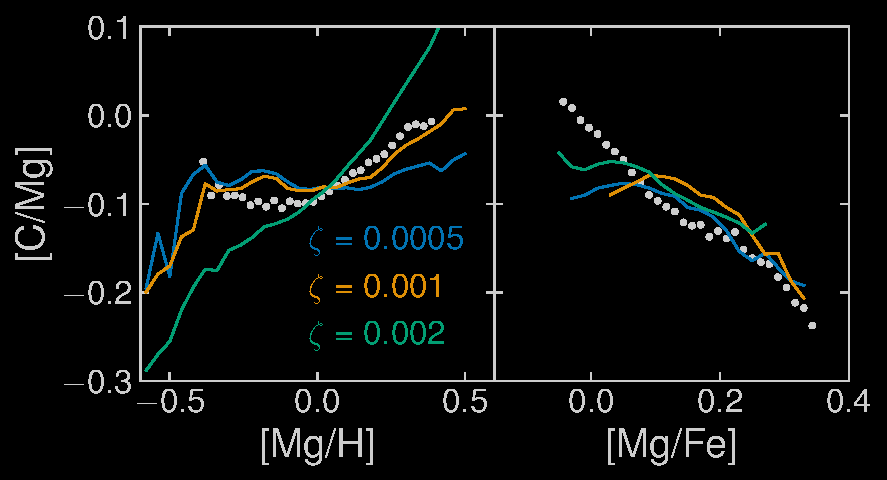
\includegraphics{beta.pdf}
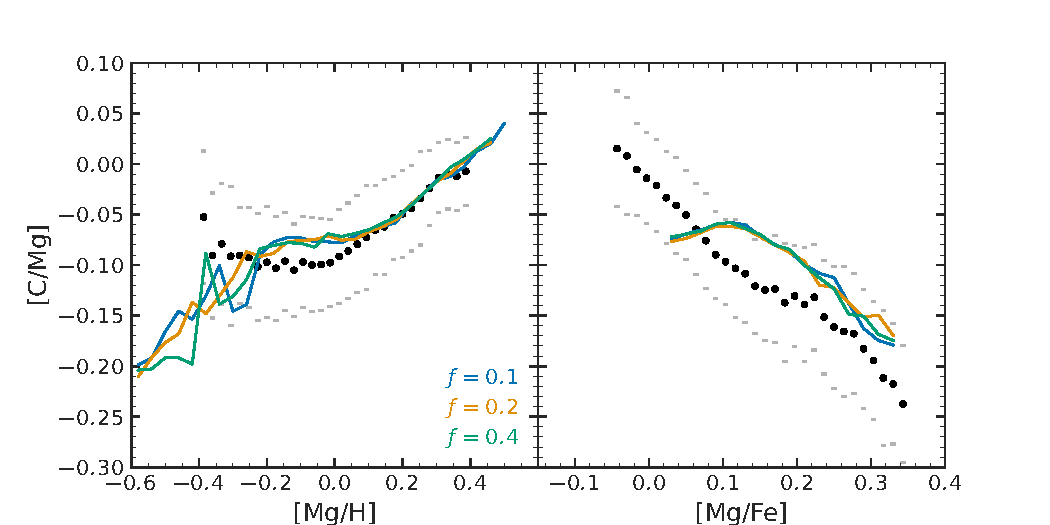
\includegraphics{f_agb.pdf}

\caption[Adjusted yield models]{Similar to \ref{fig:agb_sims} except the top plot shows the fiducial model with lower and higher values of $\beta$, the C-CCSNe metallicity dependence. The bottom plot is the same except shows varying AGB fractions.}
\end{figure}

The next question is how does changing the CCSNe carbon yield affect the model?
We now consider variations of our fiducial model:
\begin{itemize}
    \item $f_{\rm agb} = 0.2$
    \item AGB model: \cristallo
    \item $Z_{\rm C}^{\rm cc} = 0.004 (Z/Z_{\sun })^{0.4}$ ($\beta = 4$)
\end{itemize}

We could chose to vary the value of $\alpha$; however, the overall scaling of
yields is unknown so our constraint is really that $Y_{\rm C}/Y_{\rm O} =
0.dfsjkhld$, based on binning from our data. As discussed in the previous
section, we chose to leave the total value of the IMF integrated yield fixed,
and then assert the AGB fraction (next section) and scale the AGB yields from
literature appropriety. As such, 

As we display in Fig. \ref{fig:beta_f}, we observe that changes in $\beta$ are
approprietly reflected in the resulting \caah~trend. As the metallicity
dependence steepens with higher $\beta$, the [C/Mg] ratio becomes
correspondingly more dependent on [Mg/H].

Wow! Equilibrium!! See section \ref{sec:equilibrium}

Importantly, the \caafe trend is mostly unaffected by choosing a different
CCSNe yield. As all CCSNe enrichment happens at the same, rapid timescale, by
taking a slice in [Mg/H], this metallicity dependence is effectively ignored as
the only effect can be a vertical offset if the slice is narrow enough. 

So, the scaling of the trend and metallicity dependence of carbon (as seen in
the \caah~trend) gives information on the total carbon yield and the behavior
of CCSNe (as the dominating producer of carbon);
the \caafe trend exposes the delayed effect of carbon from AGB contribution.

One caveat is that the slope of this trend is also determined by the ratio of delayed iron to CCSNe iron production as well. If the SNeIa iron fraction is increased, then more iron enters later reducing the slope of the trend as AGB becomes a more rapid mechanism than Fe comparatively. The difference however is that changing the Fe franction mostly affects the tail of the distribution as this controls the speed of descent off the high $\alpha$ sequence, but the AGB fraction even changes the behavior for the low $\alpha$ sequence.

One potential tension with data is our models predict a low value for the AGB fraction of stars. 

Our model with Z-dependent CCSNe yields has $f_\text{agb} = 0.05$ which implies that CCSNe overwhelms AGB production and there should not be a seperation between low and high alpha sequences. However, V21 observes a significant seperation implying a more substantial delayed-time source. 

Even changing the AGB model does not affect the conclusion significantly. 

An alternate solution is to reduce the outflows and core collapse yields similarly, consistent with a model where more large stars collapse directly into black holes. This leaves the $y_\text{C}^\text{CC}/y_\text{O}^\text{CC}$ ratio unchanged, but because $y_\text{C}^\text{CC}$ is unchanged, the relative size of the AGB contribution is larger. 


Increasing the relative AGB production lowers the magnitude of  $y_\text{C}^\text{CC}/y_\text{O}^\text{CC}$, but the metallicity dependence of the ratio must increase to compensate for the inverse metallicity dependence of AGB carbon yields. 

These models are indistinguishable in the \caah~plane from our adjusted CCSNe model, so future work investigating the SFH and carbon isotopic ratios in more depth may be able to provide more insight. In the next section, we develop the analytic tools to explore this problem in more depth. 




\begin{figure}
\centering
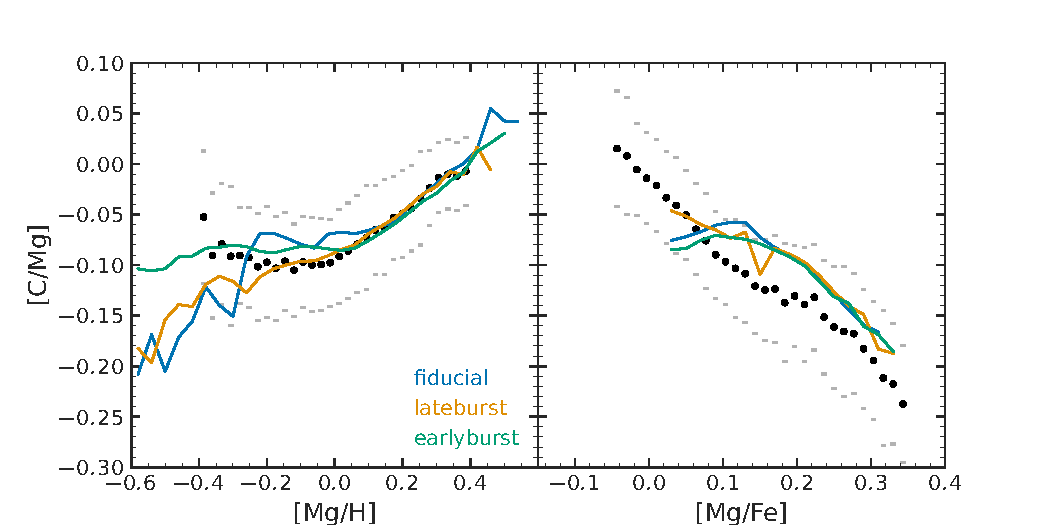
\includegraphics[]{lateburst_eta.pdf}

\caption[Lateburst and reduced-outflow models]{Same as Fig. \ref{fig:agb_sims} but comparing the fiducial model to the reduced outlow model and a lateburst model. (okay, need to totally change approach...)}
\end{figure}

We consider a simple modification of our SFH described by our lateburst model
(see Equation \ref{eq:lateburst})

equation of lateburst

However, we find that the star formation history has a negligable effect on the shape of the mean track. More drastic changes in SFH could explain the high alpha/low alpha seperation but we leave further exploration of SFH to future work. 








\section{Outflows}

In GCE there are models requiring significant mass loading, but other approaches neglect outlows altogether. (Minchev, Chiappini and Martig (13, 14), Spitoni ++ 19,20,21). 

We can modify our model to account for this by $\eta=0$. 

A common degeneracy in chemical evolution models is the yield-outflow degeneracy. An increase in stellar yields has a near-identical effect as a decrease in outflows. However, reducing the outflows reduces the evolution timescale of the system. 

The theoretical motivation for decreasing outflows is due to the uncertainty in the explodability landscape---if less massive stars explode, then both the yields and outflows will be reduced by some factor. So, when we explore reduced outflow models, we consider models where both the outflows and yields are reduced by approximately the same factor, to leave the equilibrium abundances of a pure CCSNe unchanged. 

The effect of reducing outflows is then increasing the relative contributions of non-CCSNe processes. For carbon, this increases the AGB fraction.

We have found that the \caah~relationship may provide insight into this issue. [O/Fe] is a tracer of the relative contributions of CCSNe and delayed-time sources in chemical evolution. So, the appearance of a slope in [O/Fe] implies that there is a substantial delay-time process in carbon evolution. 
The metallicity-dependence of carbon yields complicates this picture because
younger stars have higher [O/Fe] as the SNeIa contributions take up to 10Gyr,
so metal-poor young stars will naturally have lower [C/O], agreeing with the
slope observed in\caafe. However, a pure CCSNe carbon model cannot reproduce the slope accurately as  


We find that we can adjust both the outflows and scale down the yields if we change our model for $y_\text{C}^\text{CC}/y_\text{O}^\text{CC}$. For example, reducing outflows and CCSNe yields by a factor of two requires the modified parameters
$\alpha = 0.033$ and $\beta = 0.625$, which results in a slightly lower value at solar but nearly a doubling of the metallicity dependence.

\section{Understanding Scatter}

\begin{figure*}
    \centering
    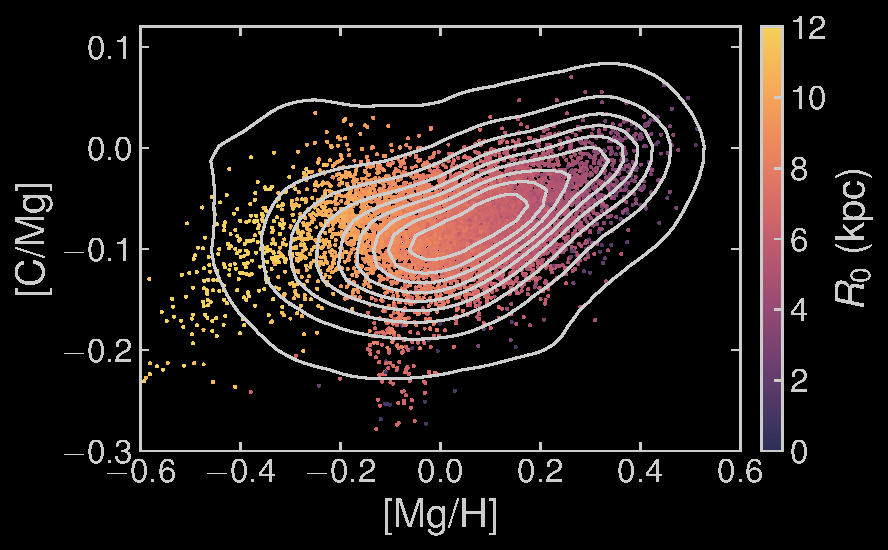
\includegraphics[scale=0.9]{cooh_scatter.pdf}
    \caption[Scatter agreement]{The simulated stars of our model at present day plotted on \caah~and colored such that lighter colors represent stars born at greater galactric radii.}
\end{figure*}

Beyond simply comparing median trends, we can compare the distribution 
shape of our distribution to observations. 

\section{Comparison to Observations}

\begin{figure*}
\centering
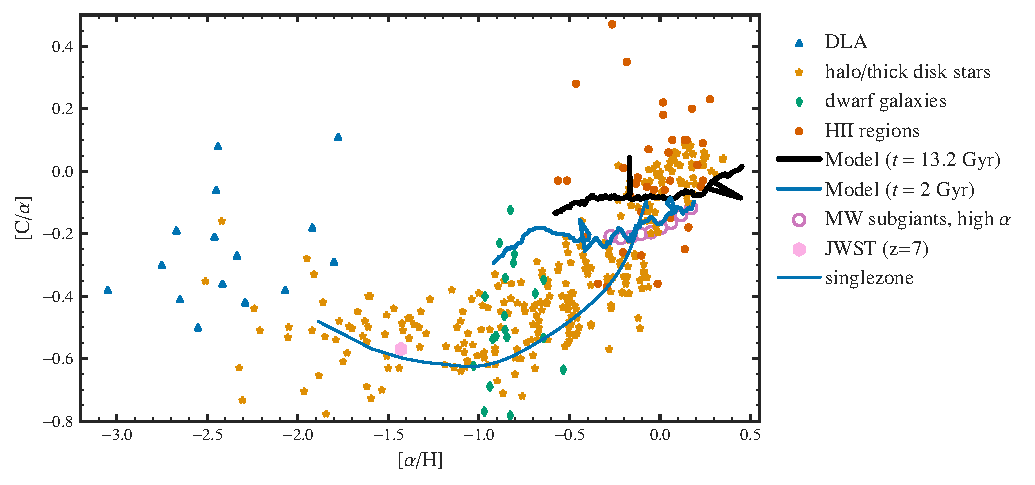
\includegraphics[]{summary.pdf}
\caption[Gas phase abundances]{Present-day gas phase tracks of the fiducial model in \caah~space. M101 is valid comparison to MW ...(van Dokkum et al. 2014)}
\label{fig:gas_phase}
\end{figure*}

Carbon measurments in stars are difficult. There are measurments which can however be used to test. 

We don't predict low metallicity but we are in agreement, substantial error bars.

Pop III stars from Cooke++. 

Beyond Milky Way stars, astronomers have observed carbon to oxygen ratios in
HII-regions through either Recombination Lines or (OTHER TEchnique0), enabling
us to probe gas-phase abundances of carbon in our galaxy and other types of
galaxies from dwarf to elliptical. 

In Fig. \ref{fig:gas_phase}, we plot our fiducial model's gas phase abundances
at present day and 2Gyr compared to C/O
abundances measured in both stars, our subgiant sample, halo stars, galaxies,
and even Damped Lynman Alpha (DLA) systems. 

Our model appears to be broadly consistant with the gas phase data, however these imply if anything that the slope should be increased. 

Are HII regions a good approximation?

Measuring carbon in the gas phase is challenging. Carbon emission lines are
very weak compared to other common lines, (visible/etc.).
Temperature/modelining limitations. Lack of strong HII calibration. 

Short discussion of measurment challenges in extragalactic galaxies, how other galaxies and dwarf SFH may come into play, why this relation is notecably steeper.

Our model fails to capture the trend past [$\alpha$/H]$=-1$. As our knowledge
of stellar evolution is limited, our knowledge of extremely metal poor stellar
evolution is extremely limited. (despite a pure H/He born star appearing
simpler lolol). A variety of explanation for the increasing relative carbon
enrichments for metal-poor stars have been proposed (e.g. ...). The likely case
that Population III star supernovae produced high abundances of carbon seems
most plausable, especially given our uncertainty in the carbon yields and the
short timescales required to create this enhancement (e.g. $z\sim 2$ DLA,
dwarfs, etc.) make it unlikely that AGB stars could be the culprit. 

As any constraints in this regieme are poor, we choose to only qualitatively
conclude that CCSNe carbon production increases at extremely low metallicity
but the details of this remains an open question.


Can we use our yield estimations and apply them to extragalactic sources successfully? 

Explain Berg+19,

Bursty SFH may not be needed to explain scatter as the C/O slope + differet evolutionary timescales is capable alone of reproducing this scatter.

While the extragalactic trend appears to be more steeply sloped than our models, this is because of ***e.g. mass-dependent outflow rates/differening SFH between galaxies. 


\chapter{Conclusions}

\begin{itemize}
    \item James ++23 Nitrogen,
    \item J++ found yield ratios, APOGEE -> yield assumptions
    \item SFH and eta don't matter too much.

        \item
        \item Variations in f and beta
        \item Evolutionary history
        \item Gas phase and Pop III
        \item Implications in Stellar evolution
        \item Continuing to work on neutron-capture e.t.c., 
        \item MWM and value of this work
\end{itemize}

Directions-->SneIa/AGB trends as a constraint on DTD.
Observations of Carbon in metal poor stars, extragalactic (call out any
existing surveys in e.g. APOGEE/DESI?)
Abundance ratios (e.g.C12/C13) as additional constraints


The Acknowledgements section is not numbered. Here you can thank helpful
colleagues, acknowledge funding agencies, telescopes and facilities used etc.
Try to keep it short.

Numpy, pandas, scipy, VICE, matplotlib
\cite{numpy, matplotlib}

\cite{OhioSupercomputerCenter1987}


%%%%%%%%%%%%%%%%%%%% REFERENCES %%%%%%%%%%%%%%%%%%

% The best way to enter references is to use BibTeX:

\newpage
\bibliographystyle{aasjournal}
\addcontentsline{toc}{chapter}{Bibliography}
\bibliography{main} % if your bibtex file is called example.bib


% Alternatively you could enter them by hand, like this:
% This method is tedious and prone to error if you have lots of references
%\begin{thebibliography}{99}
%\bibitem[\protect\citeauthoryear{Author}{2012}]{Author2012}
%Author A.~N., 2013, Journal of Improbable Astronomy, 1, 1
%\bibitem[\protect\citeauthoryear{Others}{2013}]{Others2013}
%Others S., 2012, Journal of Interesting Stuff, 17, 198
%\end{thebibliography}

%%%%%%%%%%%%%%%%%%%%%%%%%%%%%%%%%%%%%%%%%%%%%%%%%%

%%%%%%%%%%%%%%%%% APPENDICES %%%%%%%%%%%%%%%%%%%%%

\appendix
\chapter*{Appendix}
\addcontentsline{toc}{chapter}{Appendix}
\renewcommand{\thesection}{A.\arabic{section}}
\renewcommand\thefigure{A.\arabic{figure}}    
\setcounter{figure}{0}



\section{Validating the APOGEE Subgiant Sample}\label{sec:jack}
Our APOGEE subgiant sample excludes stars marked with the following flags:
\begin{itemize}
\item \texttt{ancillary young embedded cluster}
\item \texttt{ancillary emission line star}
\item \texttt{MIR-deected candidate cluster member}
\item \texttt{selected as part of the EB program}
\item \texttt{selected as part of the young cluster study (in-SYNC)}
\item \texttt{W3/4/5 star forming complex}
\end{itemize}

To select stars only in the subgiant branch, we select stars in a polygon in $\log g$-$T_\text{eff}$ space described by the following cuts:
\begin{equation}
\begin{cases}
\log g \geq 3.5 \\
\log g \leq 0.004\ T_\text{eff} - 15.7 \\
\log g \leq 0.00070588\ T_\text{eff} + 0.358836 \\
\log g \leq -0.0015\ T_\text{eff} + 12.05 \\
\log g \geq 0.0012\ T_\text{eff} - 2.8 \\
\end{cases}
\end{equation}

Instead of excluding stars which have experienced FDU and thus modified carbon abundances as JACK's subgiant sample does, another approach to predict the birth abundances of carbon and nitrogen in stars is to model the predicted abundance effects of dredge up and then correct the measured abundances, as is done in V21. 


\newpage
\section{Effects of Alternate AGB Models}\label{sec:alt_agb}


While we focus the main discussion of the paper on the C11 model, other AGB models can have notable effects on abundance trends at ***

Because the predictions of the AGB yield models we consider are dwarfed by the
required CCSNe carbon production to match observations (see Fig. ***), we briefly explore here the effects of variations in AGB models affect abundance trend predictions when these models are amplified to match observational [C/MG]-[Mg/Fe] trends. 

While most models are well represented by our AGB-fraction formalism, V13 presents a challenge as the predicted solar yield is much lower than the lower metallicity predictions, requiring the solar value to be a certain fraction forces us to amplify the yields by an unreasonable about (of order 10-30times) to reach the same $f_{\rm AGB}$ as other models. Thus, we instead calculate $f_{\rm AGB}$ at a metallicity of ... for this model. 

V13 is also interesting as at high metallicity, the yields quickly become strongly negative. This causes a reversal of the [C/Mg]-[Mg/Fe] trend at high [Mg/H] slices (figure ...). As our set of observations do not appear to reverse, this indicates that carbon yields likely stay positive even at slightly super-solar, so models like V13 are a poor match to observations. 
Plot of age metallicity relationship?


\begin{figure}[htp]
    \includegraphics{coofe_agb_extra.pdf}
    \includegraphics{coofe_agb_extra_0.2.pdf}

    \caption[Alternate AGB models]{Same as \ref{fig:agb_sims} but comparing our fiducial model to our recommended z-dependent $y_\text{C}^\text{CC}$ model. A plot of the stars of our favored CCSNe model colored by radius. The contours represent the density of V+21 data. The model is given Gaussian scatter equivalent to the mean error in the abundances reported by APOGEE. }
\end{figure}




\label{lastpage}
\end{document}




